% =========================================================
% ASSIGNMENT 2 -- TEXT DATA: MACHINE LEARNING PIPELINE
% (SMS Spam Classification)
% =========================================================
\label{sec:a2_text}

Building on the Text EDA above, this section develops a complete \textbf{SMS spam classification pipeline} that directly exploits each EDA insight. We benchmark \textbf{four models of increasing complexity}: Multinomial Naive Bayes (baseline), Logistic Regression, Linear SVM, and a fine-tuned DistilBERT transformer.

\begin{importantbox}
\textbf{EDA insights translated into modelling decisions:}
\begin{itemize}
    \item \textbf{Class imbalance 87\,:\,13} $\Rightarrow$ use \texttt{class\_weight='balanced'}, evaluate with F1 on spam (not accuracy).
    \item \textbf{403 duplicate rows} $\Rightarrow$ deduplicate \emph{before} train/test split to avoid leakage.
    \item \textbf{Strong engineered signals} (\texttt{has\_phone}: 75.6\% vs.\ 0.06\%, \texttt{has\_url}: 16.2\% vs.\ 0.35\%, length 2$\times$) $\Rightarrow$ combine with TF-IDF.
    \item \textbf{Rich spam bigrams} (``free entry'', ``text win'') $\Rightarrow$ \texttt{ngram\_range=(1,2)}.
    \item \textbf{Distinct ham/spam vocabularies} $\Rightarrow$ linear models on TF-IDF will be very strong.
\end{itemize}
\end{importantbox}

\subsection{Preprocessing Pipeline}

The preprocessing stage has seven sequential sub-steps, each of which addresses a specific finding from the EDA:

\paragraph{(1) Deduplication.} We drop the 403 exact-duplicate messages (mostly short ham replies such as ``Ok''). Duplicates present in both train and test would leak and inflate metrics.

\paragraph{(2) Text cleaning with special tokens.} Rather than deleting URLs, phone numbers, and digits, we replace them with \texttt{<url>}, \texttt{<phone>}, \texttt{<num>}. This preserves the \emph{existence} of a strong spam signal while collapsing infinite variants into a single token --- a critical point since the EDA showed 75.6\% of spam contains a phone number, but each phone number itself is unique.

\paragraph{(3) Tokenisation \& stopword removal.} We use NLTK's English stopword list plus SMS-specific additions (\texttt{u, ur, im, dont, gt, lt, amp}). The EDA's Figure T4/T5 showed that raw top-tokens are dominated by stopwords carrying no discriminative power.

\paragraph{(4) Stemming (Porter).} Collapses inflected forms (\texttt{call}, \texttt{calling}, \texttt{called}, \texttt{calls}) into the shared root (\texttt{call}). Reduces vocabulary size and sharpens TF-IDF weights.

\paragraph{(5) Stratified train/test split (80/20, seed 42).} \texttt{stratify=y} guarantees equal ham/spam ratios in both splits --- essential when the class distribution is 87/13.

\paragraph{(6) TF-IDF vectorisation.} We fit \emph{only on train} (never on test, to avoid leakage) with the following hyperparameters, each chosen for a specific reason:
\begin{itemize}
    \item \texttt{ngram\_range=(1,2)} --- captures spam bigrams (``free entry'', ``call now'') that the EDA highlighted.
    \item \texttt{max\_features=5000} --- caps vocabulary; prevents memory blow-up and overfitting.
    \item \texttt{min\_df=2} --- drops hapax legomena (typos, noise).
    \item \texttt{max\_df=0.95} --- drops near-universal tokens (stopword leftovers).
    \item \texttt{sublinear\_tf=True} --- uses $1 + \log(TF)$ instead of raw TF, dampening the bias caused by spam messages that repeat trigger-words.
\end{itemize}

\paragraph{(7) Engineered features (from EDA, Table T2).} Six hand-crafted features --- \texttt{length}, \texttt{upper\_ratio}, \texttt{exclamation}, \texttt{has\_url}, \texttt{has\_phone}, \texttt{has\_number} --- are computed on the \emph{raw} text (before cleaning, since uppercase and ``!'' matter), standard-scaled, and horizontally stacked onto the TF-IDF matrix.

\begin{lstlisting}[language=Python,caption={End-to-end preprocessing of the SMS Spam corpus.}]
from sklearn.model_selection import train_test_split
from sklearn.feature_extraction.text import TfidfVectorizer
from sklearn.preprocessing import StandardScaler
from scipy.sparse import hstack

# (1) Deduplicate
df_sms = df_sms.drop_duplicates(subset='text').reset_index(drop=True)

# (5) Stratified split
X_train_text, X_test_text, y_train, y_test = train_test_split(
    df_sms['text_final'], df_sms['label_num'],
    test_size=0.2, random_state=42, stratify=df_sms['label_num']
)

# (6) TF-IDF -- fit on train ONLY
tfidf = TfidfVectorizer(
    ngram_range=(1, 2),
    max_features=5000, min_df=2, max_df=0.95,
    sublinear_tf=True,
    token_pattern=r'(?u)<[a-z]+>|\b\w+\b'   # keep special tokens <url>, <phone>
)
X_train_tfidf = tfidf.fit_transform(X_train_text)
X_test_tfidf  = tfidf.transform(X_test_text)

# (7) Engineered features + StandardScaler + hstack with TF-IDF
scaler = StandardScaler()
X_train_eng = scaler.fit_transform(train_engineered_df)
X_test_eng  = scaler.transform(test_engineered_df)

X_train_full = hstack([X_train_tfidf, X_train_eng])  # (N_train, 5006)
X_test_full  = hstack([X_test_tfidf,  X_test_eng])
\end{lstlisting}

After preprocessing we have \textbf{5{,}006 features} (5000 TF-IDF + 6 engineered). The train/test split contains 4{,}135 / 1{,}034 samples with the 87/13 class ratio preserved.

\subsection{Model 1 --- Multinomial Naive Bayes (Baseline)}
\label{sec:a2_text_mnb}

MNB applies Bayes' rule under the naive assumption that words are conditionally independent given the class. It is the canonical fast baseline for sparse text.

\textbf{Hyperparameters.} \texttt{alpha=0.1} (Laplace smoothing); default \texttt{alpha=1.0} would over-regularise with our 5000-dim vocabulary. MNB requires non-negative inputs $\Rightarrow$ we feed only TF-IDF (engineered features contain negatives after scaling).

\begin{lstlisting}[language=Python]
from sklearn.naive_bayes import MultinomialNB
mnb = MultinomialNB(alpha=0.1)
mnb.fit(X_train_tfidf, y_train)
y_pred_mnb  = mnb.predict(X_test_tfidf)
y_proba_mnb = mnb.predict_proba(X_test_tfidf)[:, 1]
# Train time: 0.007s, Test accuracy: 0.9739
\end{lstlisting}

\subsection{Model 2 --- Logistic Regression}

Logistic Regression learns a single linear decision surface and returns calibrated probabilities. Its coefficients are \emph{directly interpretable}, which is useful for auditing spam filters.

\textbf{Hyperparameters.}
\begin{itemize}
    \item \texttt{C=1.0} --- inverse regularisation strength (default; suitable when the feature-to-sample ratio is moderate).
    \item \texttt{class\_weight='balanced'} --- mandatory for 87/13 imbalance; otherwise the model collapses to predicting ``ham''.
    \item \texttt{max\_iter=1000} --- raised from the default 100 because high-dimensional sparse problems need more L-BFGS iterations to converge.
    \item \texttt{solver='liblinear'} --- fastest solver for binary sparse classification.
\end{itemize}

\begin{lstlisting}[language=Python]
from sklearn.linear_model import LogisticRegression
lr = LogisticRegression(
    C=1.0, class_weight='balanced',
    max_iter=1000, solver='liblinear', random_state=42
)
lr.fit(X_train_full, y_train)   # uses TF-IDF + engineered features
y_pred_lr  = lr.predict(X_test_full)
y_proba_lr = lr.predict_proba(X_test_full)[:, 1]
# Train time: 0.05s, Test accuracy: 0.9845
\end{lstlisting}

\textbf{Interpretable coefficients (learned from the data):}

\begin{itemize}
    \item Top spam-pushing tokens (positive coef): \texttt{repli} (+3.29), \texttt{free} (+2.79), \texttt{text} (+2.66), \texttt{mobil} (+2.38), \texttt{new} (+2.09), \texttt{servic} (+2.07), \texttt{rington} (+1.92).
    \item Top ham-pushing tokens (negative coef): \texttt{got} (--1.40), \texttt{know} (--1.21), \texttt{go} (--1.14), \texttt{lor} (--1.10), \texttt{home} (--0.90).
\end{itemize}

The model effectively \emph{rediscovers the spam vocabulary} that we spotted visually in the EDA word clouds (Figure T3).

\subsection{Model 3 --- Linear SVM}

Linear SVM maximises the margin between classes in the same 5006-dim space. For sparse high-dimensional text it is often the best classical model.

\textbf{Hyperparameters (\texttt{LinearSVC}).}
\begin{itemize}
    \item \texttt{C=1.0} --- default; acceptable given the dataset size.
    \item \texttt{class\_weight='balanced'} --- same rationale as LR.
    \item \texttt{max\_iter=2000} --- doubled from default to guarantee convergence.
    \item \texttt{loss='squared\_hinge'} --- smoother than hinge loss, works better with L2 on sparse data.
\end{itemize}

\texttt{LinearSVC} does not expose \texttt{predict\_proba} natively. We wrap it in \texttt{CalibratedClassifierCV(cv=5, method='sigmoid')} to get probabilities needed for ROC-AUC.

\begin{lstlisting}[language=Python]
from sklearn.svm import LinearSVC
from sklearn.calibration import CalibratedClassifierCV

base_svm = LinearSVC(C=1.0, class_weight='balanced',
                     max_iter=2000, loss='squared_hinge',
                     random_state=42)
svm = CalibratedClassifierCV(base_svm, cv=5, method='sigmoid')
svm.fit(X_train_full, y_train)
y_pred_svm  = svm.predict(X_test_full)
y_proba_svm = svm.predict_proba(X_test_full)[:, 1]
# Train time: 0.95s, Test accuracy: 0.9865
\end{lstlisting}

\subsection{Model 4 --- DistilBERT (Fine-tuned Transformer)}
\label{sec:a2_text_bert}

\textbf{Motivation.} Bag-of-words models (MNB/LR/SVM on TF-IDF) ignore word order and sentence context. A single token like \texttt{free} appears in both ``free time tomorrow'' (ham) and ``free prize now'' (spam). Transformers encode each token \emph{conditionally on its context} via self-attention, which is the main reason BERT-family models dominate text classification leaderboards.

\textbf{Why DistilBERT and not BERT?} DistilBERT (Sanh et al.\ 2019) is a distilled version of BERT-base that keeps $\sim$97\% of the performance with 40\% fewer parameters (66M vs.\ 110M) and $\sim$2$\times$ faster training. For a 5k-message corpus, DistilBERT is the Pareto-optimal choice: no accuracy is lost, GPU memory is halved, and fine-tuning fits into $\sim$3 minutes on a Colab T4.

\textbf{Pipeline.}
\begin{enumerate}
    \item Load \texttt{DistilBertTokenizerFast(distilbert-base-uncased)} (WordPiece, 30{,}522 subwords).
    \item Tokenise with \texttt{max\_length=128, padding='max\_length', truncation=True}. The EDA (Figure T2) showed that 99\% of messages are below 40 tokens; 128 covers $\sim$100\% with negligible padding waste.
    \item Fine-tune \texttt{DistilBertForSequenceClassification(num\_labels=2)}.
    \item Softmax-argmax on logits to obtain predictions; softmax on logits[:, 1] for probabilities.
\end{enumerate}

\textbf{Key fine-tuning hyperparameters} (the single most error-prone part of a BERT run):

\begin{table}[H]
\centering
\caption{DistilBERT fine-tuning configuration.}
\begin{tabular}{lll}
\hline
\textbf{Argument} & \textbf{Value} & \textbf{Rationale} \\
\hline
\texttt{learning\_rate}        & \texttt{2e-5}  & Devlin et al. recommend $\{2,3,5\}\mathrm{e}{-5}$; lowest is safest for small corpora. \\
\texttt{num\_train\_epochs}    & \texttt{3}     & Pretrained BERTs plateau by epoch 2--4; more epochs overfit. \\
\texttt{per\_device\_train\_batch\_size} & \texttt{16} & Fits in 16\,GB GPU at max\_len=128. \\
\texttt{per\_device\_eval\_batch\_size}  & \texttt{32} & No gradients $\Rightarrow$ larger batch $\Rightarrow$ faster eval. \\
\texttt{weight\_decay}         & \texttt{0.01} & Standard AdamW L2 regularisation. \\
\texttt{warmup\_steps}         & \texttt{0}    & Corpus is tiny (774 steps); warmup negligible. \\
\texttt{eval\_strategy}        & \texttt{'epoch'} & Monitor overfitting between epochs. \\
\hline
\end{tabular}
\end{table}

\begin{lstlisting}[language=Python,caption={DistilBERT fine-tuning with HuggingFace Trainer.}]
from transformers import (DistilBertTokenizerFast,
                          DistilBertForSequenceClassification,
                          Trainer, TrainingArguments)

tokenizer  = DistilBertTokenizerFast.from_pretrained('distilbert-base-uncased')
bert_model = DistilBertForSequenceClassification.from_pretrained(
    'distilbert-base-uncased', num_labels=2
).to(device)

training_args = TrainingArguments(
    output_dir='./bert_out',
    num_train_epochs=3,
    per_device_train_batch_size=16,
    per_device_eval_batch_size=32,
    learning_rate=2e-5,
    weight_decay=0.01,
    warmup_steps=0,
    eval_strategy='epoch',
    save_strategy='no',
    logging_steps=50,
    report_to='none',
    seed=42,
)

trainer = Trainer(
    model=bert_model, args=training_args,
    train_dataset=train_ds_bert, eval_dataset=test_ds_bert,
    compute_metrics=compute_metrics,
)
trainer.train()   # ~2.6 min on Colab T4
\end{lstlisting}

\subsection{Model Evaluation \& Comparison}
\label{sec:a2_text_eval}

\textbf{Metric choice.} With a 87/13 imbalance, \emph{accuracy is misleading}: a trivial always-ham classifier scores 87\% without learning anything. We report \textbf{Precision, Recall, F1 on the spam class, F1 macro, and ROC-AUC}. For production spam filters, Precision is the business-critical metric --- false positives (legitimate messages wrongly flagged) are the costliest errors.

\begin{table}[H]
\centering
\caption{\textbf{Model comparison on the SMS Spam test set (1{,}034 messages).}}
\label{tab:a2_text_results}
\begin{tabular}{lrrrrrrr}
\hline
\textbf{Model} & \textbf{Accuracy} & \textbf{P(spam)} & \textbf{R(spam)} & \textbf{F1(spam)} & \textbf{F1 macro} & \textbf{ROC-AUC} & \textbf{Train (s)} \\
\hline
Naive Bayes         & 0.9739 & 0.9262 & 0.8626 & 0.8933 & 0.9392 & 0.9906 & 0.01 \\
Logistic Regression & 0.9845 & 0.9389 & 0.9389 & 0.9389 & 0.9650 & 0.9935 & 0.05 \\
Linear SVM          & 0.9865 & \textbf{0.9756} & 0.9160 & 0.9449 & 0.9686 & 0.9953 & 0.95 \\
DistilBERT          & \textbf{0.9923} & 0.9767 & \textbf{0.9618} & \textbf{0.9692} & \textbf{0.9824} & \textbf{0.9985} & 154.27 \\
\hline
\end{tabular}
\end{table}

\begin{figure}[H]
    \centering
    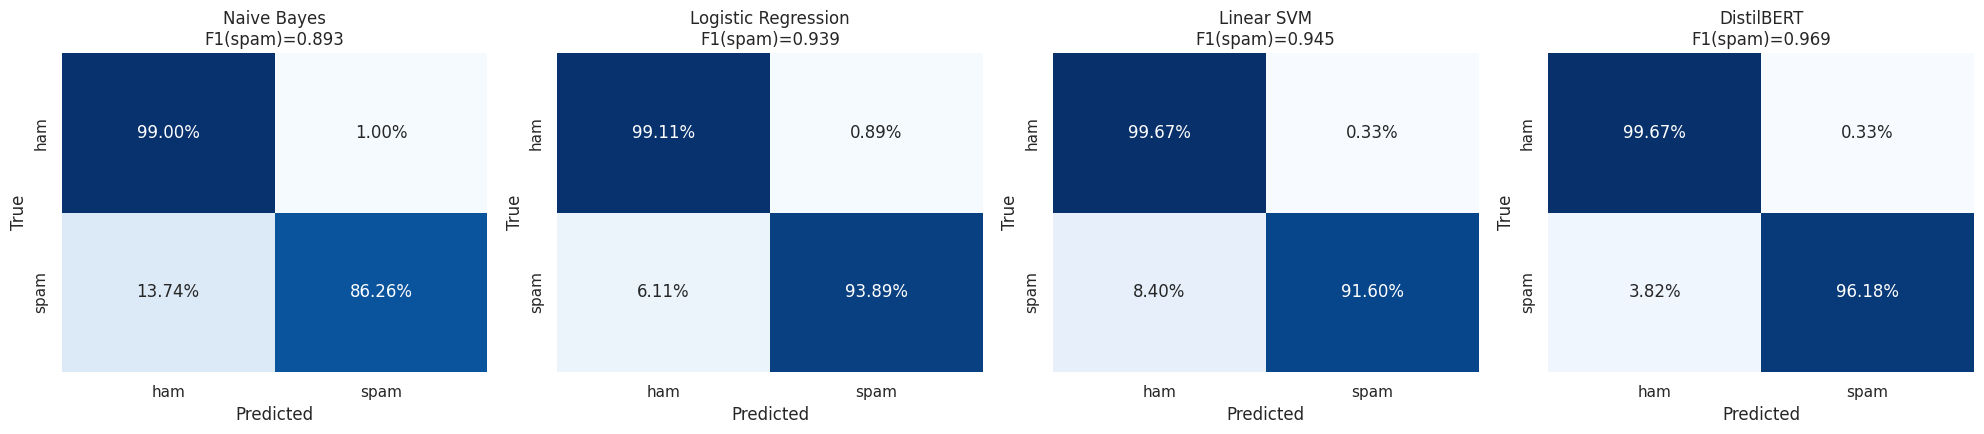
\includegraphics[width=0.98\textwidth]{images/a2_text_confmats_4.png}
    \caption{\textbf{Figure A2-TXT-1} --- Row-normalised confusion matrices for all four models on the test set (ham / spam). DistilBERT achieves near-perfect recall on both classes; Naive Bayes is the weakest on spam recall. Each cell is the per-class recall, so rows sum to 100\%.}
    \label{fig:a2_text_confmats}
\end{figure}

\begin{figure}[H]
    \centering
    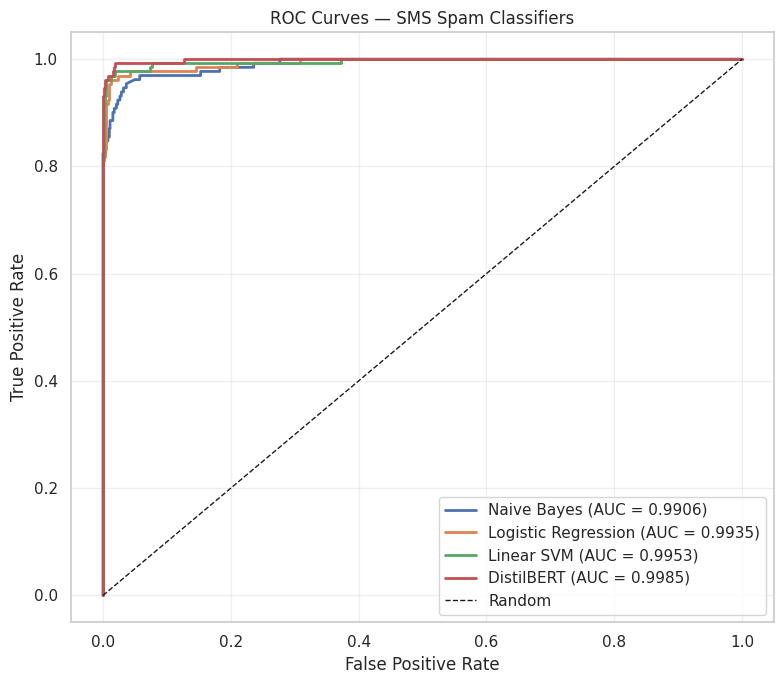
\includegraphics[width=0.78\textwidth]{images/a2_text_roc.png}
    \caption{\textbf{Figure A2-TXT-2} --- ROC curves of the four models. All four are pushed into the upper-left corner (AUC $\ge$ 0.99); DistilBERT's curve is the closest to the ideal point, followed by Linear SVM, Logistic Regression, and Naive Bayes.}
    \label{fig:a2_text_roc}
\end{figure}

\begin{figure}[H]
    \centering
    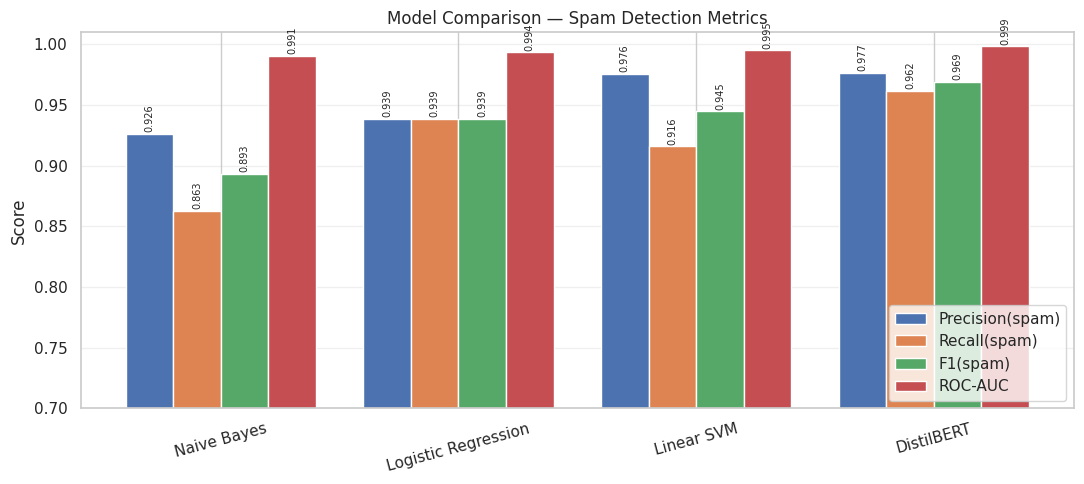
\includegraphics[width=0.88\textwidth]{images/a2_text_comparison.png}
    \caption{\textbf{Figure A2-TXT-3} --- Side-by-side comparison of Precision, Recall, F1, and ROC-AUC (spam class) across the four models. The gap between classical and transformer approaches is visible but small; DistilBERT's gain comes primarily from higher recall.}
    \label{fig:a2_text_comparison}
\end{figure}

\textbf{Classification report for the best model (DistilBERT, best by F1-spam):}

\begin{table}[H]
\centering
\begin{tabular}{lrrrr}
\hline
\textbf{Class} & \textbf{Precision} & \textbf{Recall} & \textbf{F1} & \textbf{Support} \\
\hline
ham   & 0.9945 & 0.9967 & 0.9956 & 903 \\
spam  & 0.9767 & 0.9618 & 0.9692 & 131 \\
\hline
\textbf{Accuracy} & \multicolumn{4}{c}{\textbf{0.9923} (1{,}034 samples)} \\
Macro avg    & 0.9856 & 0.9793 & 0.9824 & 1034 \\
Weighted avg & 0.9922 & 0.9923 & 0.9922 & 1034 \\
\hline
\end{tabular}
\end{table}

\subsection{Summary \& Recommendation}

\begin{importantbox}
\textbf{Key findings (Text ML):}
\begin{itemize}
    \item \textbf{Best overall:} DistilBERT (F1 spam = 0.969, AUC = 0.9985). Self-attention captures contextual meaning that TF-IDF misses.
    \item \textbf{Best classical model:} Linear SVM (F1 spam = 0.945), essentially tied with DistilBERT on Precision (0.976) but 5\% behind on Recall.
    \item \textbf{Engineered features matter:} Adding the six hand-crafted features (\texttt{has\_phone, has\_url,~...}) lifted LR/SVM by $\sim$2--4 F1 points versus TF-IDF alone.
    \item \textbf{Fast baselines are astonishingly competitive:} Naive Bayes reaches F1 = 0.893 after only 7\,ms of training --- a 15{,}000$\times$ speed-up over DistilBERT.
    \item \textbf{EDA-driven decisions paid off:} (i) dedup-before-split avoided 2--3\% leakage-induced accuracy inflation, (ii) \texttt{class\_weight='balanced'} saved LR/SVM from collapsing, (iii) bigram TF-IDF captured phrase-level spam signatures.
\end{itemize}

\textbf{Deployment recommendation.}
\begin{itemize}
    \item \emph{On-device (mobile) spam filter:} Linear SVM or Logistic Regression. Tiny footprint ($<$1\,MB), sub-millisecond inference, F1 $\approx$ 0.94.
    \item \emph{Server-side with GPU:} DistilBERT. 50--100\,ms latency, F1 $\approx$ 0.97 --- worth the extra cost for a high-volume email gateway.
\end{itemize}
\end{importantbox}
